\documentclass[11pt]{article}

\usepackage{xeCJK}
\setCJKmainfont{STSong}
\setCJKsansfont{Heiti SC}

\input{../../templates/template.LaTeX.homework/structure.tex}

%----------------------------------------------------------------------------------------
%  ASSIGNMENT INFORMATION
%----------------------------------------------------------------------------------------
\newcommand{\assignmentQuestionName}{习题}
\newcommand{\assignmentClass}{离散数学}
\newcommand{\assignmentTitle}{第3章 关系 — 第10次作业}
\newcommand{\assignmentAuthorName}{乐绎华}
\newcommand{\studentID}{23363017}
\newcommand{\assignmentClassInstructor}{左孝凌、刘永才《离散数学》}
\newcommand{\assignmentDueDate}{}

\begin{document}

\maketitle
\thispagestyle{empty}
\newpage

%----------------------------------------------------------------------------------------
%  3-12(1) 整除偏序关系图
%----------------------------------------------------------------------------------------

\begin{question}{3-12(1) 整除偏序关系图}
  设集合为 $\{3,5,15\}$，$\{1,2,3,6,12\}$，$\{3,9,27,54\}$，偏序关系为整除，画出这些集合的偏序关系图，并指出哪些是全序关系。

  \begin{answer}
    \vspace{1em}
    \noindent\textbf{（1）集合 $A_1 = \{3,5,15\}$，整除关系：}

    偏序关系：$3 \mid 3$，$5 \mid 5$，$15 \mid 15$，$3 \mid 15$（因为 $15 = 3 \times 5$），$5 \mid 15$。

    哈斯图：
    \begin{center}
      \begin{tikzpicture}[scale=0.8]
        \node (15) at (0,2) {15};
        \node (3) at (-1,0) {3};
        \node (5) at (1,0) {5};
        \draw (15) -- (3);
        \draw (15) -- (5);
      \end{tikzpicture}
    \end{center}

    $3$ 与 $5$ 之间没有整除或被整除关系，故\textbf{不是全序关系}。

    \vspace{1em}
    \noindent\textbf{（2）集合 $A_2 = \{1,2,3,6,12\}$，整除关系：}

    偏序关系：$1 \mid 1,2,3,6,12$；$2 \mid 2,6,12$；$3 \mid 3,6,12$；$6 \mid 6,12$；$12 \mid 12$。

    哈斯图：
    \begin{center}
      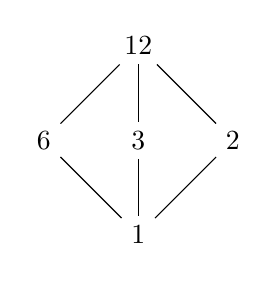
\begin{tikzpicture}[scale=0.8]
        \node (12) at (0,3) {12};
        \node (6) at (-1.5,1.5) {6};
        \node (3) at (0,1.5) {3};
        \node (2) at (1.5,1.5) {2};
        \node (1) at (0,0) {1};
        \draw (12) -- (6);
        \draw (12) -- (3);
        \draw (12) -- (2);
        \draw (6) -- (1);
        \draw (3) -- (1);
        \draw (2) -- (1);
      \end{tikzpicture}
    \end{center}

    $2$ 与 $3$ 之间没有整除关系（$2 \nmid 3$ 且 $3 \nmid 2$），故\textbf{不是全序关系}。

    \vspace{1em}
    \noindent\textbf{（3）集合 $A_3 = \{3,9,27,54\}$，整除关系：}

    偏序关系：$3 \mid 3,9,27,54$；$9 \mid 9,27$；$27 \mid 27$；$54 \mid 54$（注意 $54 = 2 \times 27$，但 $9 \nmid 54$，$27 \nmid 54$）。

    哈斯图：
    \begin{center}
      \begin{tikzpicture}[scale=0.8]
        \node (54) at (0,3) {54};
        \node (27) at (-1.5,1.5) {27};
        \node (9) at (1.5,1.5) {9};
        \node (3) at (0,0) {3};
        \draw (54) -- (27);
        \draw (54) -- (9);
        \draw (27) -- (3);
        \draw (9) -- (3);
      \end{tikzpicture}
    \end{center}

    $9$ 与 $27$ 之间没有整除关系，故\textbf{不是全序关系}。

    \vspace{1em}
    \begin{info}[结论:]
      以上三个集合上的整除偏序关系都不是全序关系。全序关系要求任意两个元素之间都有序关系，但整除关系不满足这个条件（除非集合中的元素具有链式整除关系，如 $\{1,2,4,8\}$）。
    \end{info}
  \end{answer}
\end{question}

%----------------------------------------------------------------------------------------
%  3-12(6) 偏序集的极值元与上下界
%----------------------------------------------------------------------------------------

\begin{question}{3-12(6) 偏序集的极值元与上下界}
  设集合 $P = \{x_1, x_2, x_3, x_4, x_5\}$ 上的偏序关系如图 3-12.10 所示。找出 $P$ 的最大元素、最小元素、极小元素、极大元素。找出子集 $\{x_2, x_3, x_4\}$、$\{x_3, x_4, x_5\}$ 和 $\{x_1, x_2, x_3\}$ 的上界、下界、上确界、下确界。

  \begin{figure}[htbp]
    \centering
    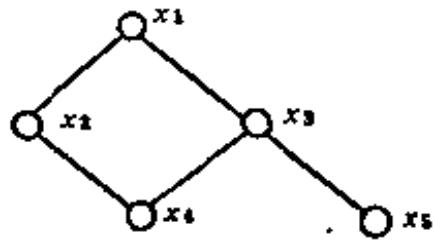
\includegraphics[width=0.4\textwidth]{fig/fig3-12-10.jpg}
    \caption{图 3-12.10 集合 $P$ 上的偏序关系}
    \label{fig:3-12-10}
  \end{figure}

  \begin{answer}
    根据图 3-12.10，$P$ 上的偏序关系哈斯图结构（由下到上）：

    \vspace{1em}
    \noindent\textbf{最大/最小/极值元素分析：}

    \begin{itemize}
      \item \textbf{最小元素}：$x_1$ 是唯一在最底层的元素，所有其他元素都 $\succeq x_1$，故 $x_1$ 是\textbf{最小元素}
      \item \textbf{最大元素}：$x_5$ 在最顶层，没有元素比 $x_5$ 大，故 $x_5$ 是\textbf{最大元素}
      \item \textbf{极小元素}：$x_1$ 是唯一没有前驱的元素，故 $\{x_1\}$ 是极小元集合
      \item \textbf{极大元素}：$x_5$ 是唯一没有后继的元素，故 $\{x_5\}$ 是极大元集合
    \end{itemize}

    \vspace{1em}
    \noindent\textbf{子集分析：}

    \begin{enumerate}
      \item \textbf{子集 $\{x_2, x_3, x_4\}$}：
        \begin{itemize}
          \item 上界：$x_5$（因为 $x_2 \preceq x_5$，$x_3 \preceq x_5$，$x_4 \preceq x_5$）
          \item 下界：$x_1$（因为 $x_1 \preceq x_2$，$x_1 \preceq x_3$，$x_1 \preceq x_4$）
          \item 上确界 (LUB)：$x_5$
          \item 下确界 (GLB)：$x_1$
        \end{itemize}

      \item \textbf{子集 $\{x_3, x_4, x_5\}$}：
        \begin{itemize}
          \item 上界：$x_5$（自身是最大上界）
          \item 下界：$x_1$（因为 $x_1 \preceq x_3$，$x_1 \preceq x_4$；注意 $x_5$ 不 $\preceq x_3$ 或 $x_4$，所以 $x_5$ 不是下界）
          \item 上确界 (LUB)：$x_5$
          \item 下确界 (GLB)：$x_1$
        \end{itemize}

      \item \textbf{子集 $\{x_1, x_2, x_3\}$}：
        \begin{itemize}
          \item 上界：$x_4$ 和 $x_5$（因为 $x_1 \preceq x_4 \preceq x_5$，$x_2 \preceq x_4 \preceq x_5$，$x_3 \preceq x_4 \preceq x_5$）
          \item 下界：$x_1$
          \item 上确界 (LUB)：$x_4$（最小上界）
          \item 下确界 (GLB)：$x_1$
        \end{itemize}
    \end{enumerate}

    \begin{info}[总结:]
      \begin{tabular}{c|c|c|c|c}
        子集 & 上界 & 下界 & 上确界 & 下确界 \\ \hline
        $\{x_2, x_3, x_4\}$ & $\{x_5\}$ & $\{x_1\}$ & $x_5$ & $x_1$ \\
        $\{x_3, x_4, x_5\}$ & $\{x_5\}$ & $\{x_1\}$ & $x_5$ & $x_1$ \\
        $\{x_1, x_2, x_3\}$ & $\{x_4, x_5\}$ & $\{x_1\}$ & $x_4$ & $x_1$
      \end{tabular}
    \end{info}
  \end{answer}
\end{question}

\end{document}
